CentralServer implementerer server-delen af systemets klient-server arkitektur. 

\begin{figure}[H]
    \centering
    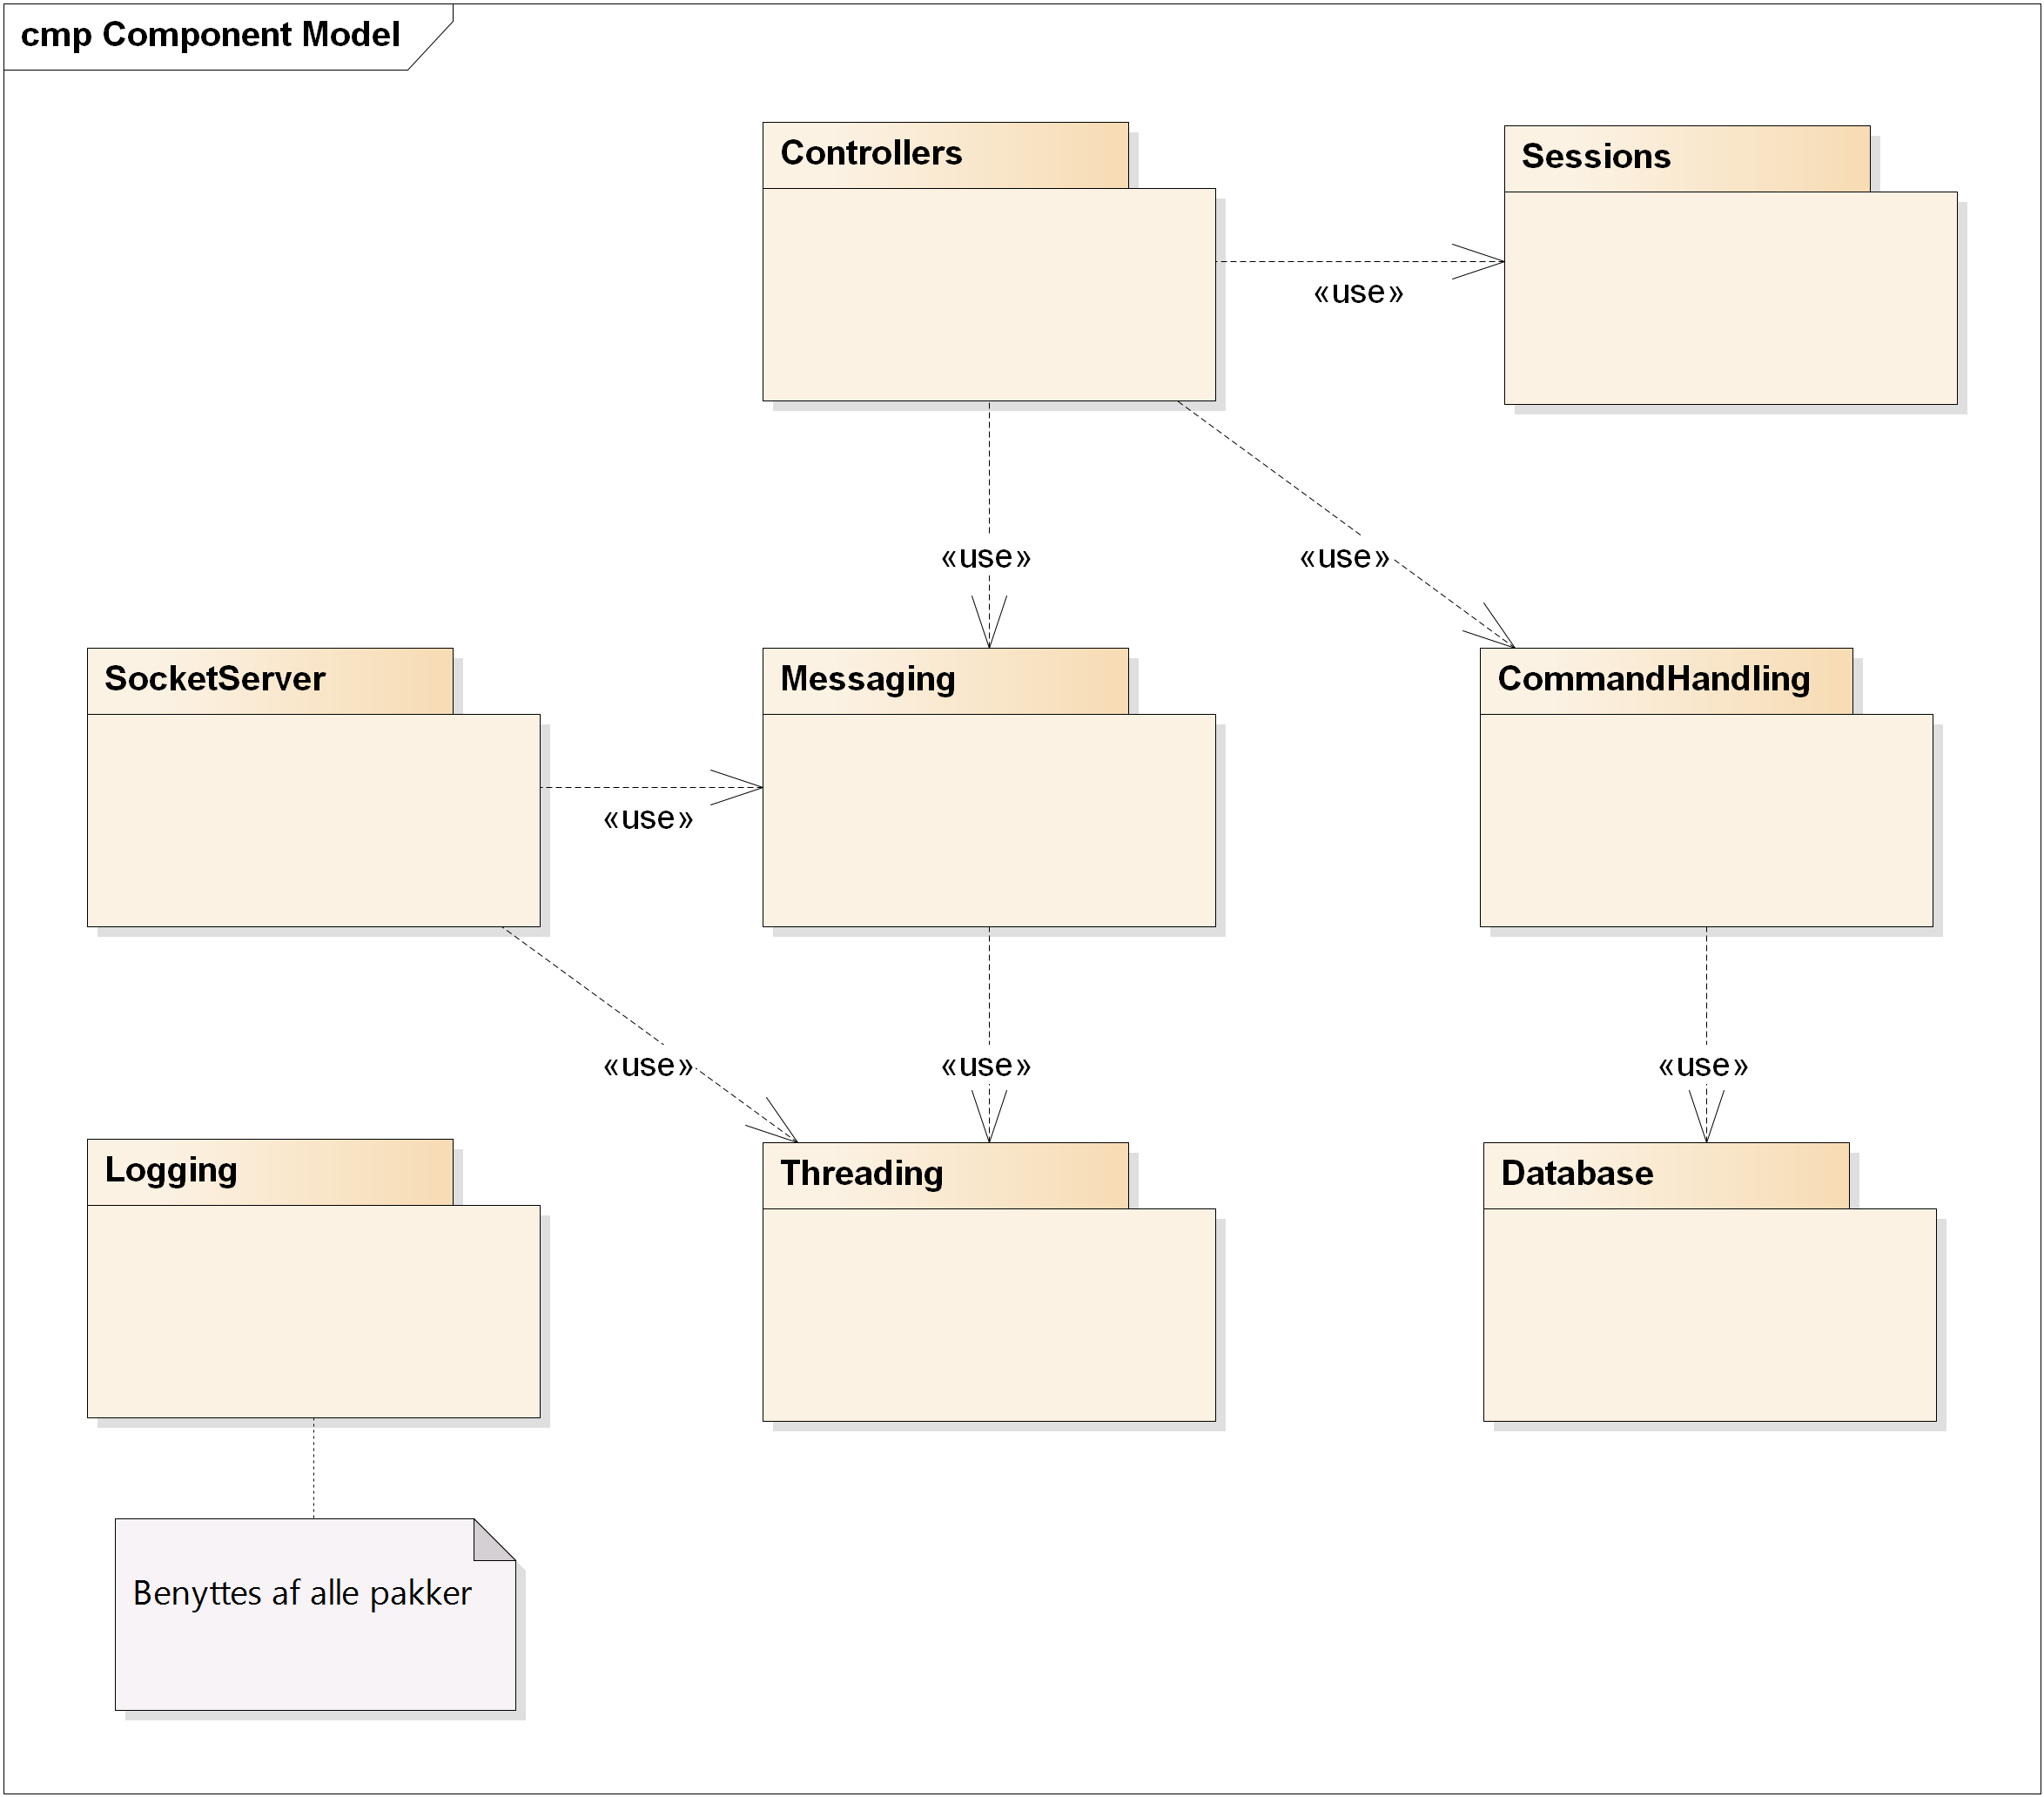
\includegraphics[width=1\textwidth]{Systemdesign/CentralServer/Images/Packages.png}
    \caption{Pakkediagram for CentralServer}
    \label{fig:CSPackages}
\end{figure}


\textbf{Controllers}\\
Indeholder implementeringerne af de forskellige tråde, der kan modtage beskeder fra andre tråde. Controllers-pakken benytter følgende pakker:

\begin{itemize}
	\item Sessions: benyttes til at identificere klienter ud fra sessions ID.
	\item Messaging: benyttes til at kunne modtage beskeder fra andre tråde.
	\item CommandHandling: benyttes til at håndtere kommandoer, som er modtaget fra forbundne klienter.
\end{itemize}

Controllers-pakken indeholder følgende:

\begin{itemize}
	\item MainControl: denne tråd står for at holde styr over, hvilke klienter, der er forbundet til serveren. Derudover benytter MainControl CommandHandling-pakken til at håndtere alle kommandoer, der modtaget fra klienter.
	\item ClientControl: denne tråd står for at læse fra - og skrive til - en klients socket-forbindelse. Der eksisterer en instans af ClientControl for hver klient, der er forbundet til serveren.
\end{itemize}


\textbf{Sessions}\\
Indeholder funktionalitet til at identificere forbundne klienter ud fra et sessions ID.\\

\textbf{Messaging}\\
Indeholder beskedsystem, som tillader tråde at kommunikere med hinanden. Denne pakke benytter Threading-pakken til at implementere en tråd, der kan modtage beskeder fra andre tråde. Alt tråd-synkronisering i CentralServer er placeret i heri.\\

\textbf{SocketServer}\\
Indeholder implementeringen af socket-serveren. Denne pakke benytter Threading-pakken til at eksekvere i en tråd, og den benytter Messaging-pakken til at sende beskeder til MainControl, når en ny klient er forbundet.\\

\textbf{CommandHandling}\\
Indeholder håndtering af kommandoer, som er modtaget fra forbundne klienter. Det er heri, at business logic er placeret. Denne pakker benytter Database-pakken til at tilgå data fra databasen.\\

\textbf{Threading}\\
Indeholder en hjælpe-klasse samt et interface, som kan benyttes til at starte tråde.\\

\textbf{Logging}\\
Indeholder funktionalitet til at logge begivenheder. Logging benyttes af alle andre pakker.\\

\textbf{Database}\\
Indeholder database access layer (DAL). Her ligger implementering af Entity Framework contexten.